\documentclass[../basic_graph_theory.tex]{subfiles}

\begin{document}
\chapter{Basic Definitions}
\setcounter{chapter}{1} %Set chapter counter
\setcounter{section}{1}
\setcounter{equation}{1}
\setcounter{figure}{1}

Some notation: $[n] = \{1,\ldots,n\}$, $V \times V$ the usual set product, $\binom{V}{2}$ denote unordered pairs of distinct elements in $V$.
%
\begin{defn}(\index{Graph}Graph).
    A (simple) graph $G$ consists of a finite vertex set $V := V(G)$ and an edge set $E := E(G) \subset \binom{V}{2}.$
\end{defn}
Before diving deeper, we first define some classes of graphs.
\begin{enumerate}
    \item \textbf{Undirected graph}: When an edge $e$ in a graph is represented by $(x,y)$ and $(x,y)=(y,x)$, then such a graph is called an undirected graph.
          \begin{figure}[hbt!]
              \centering
              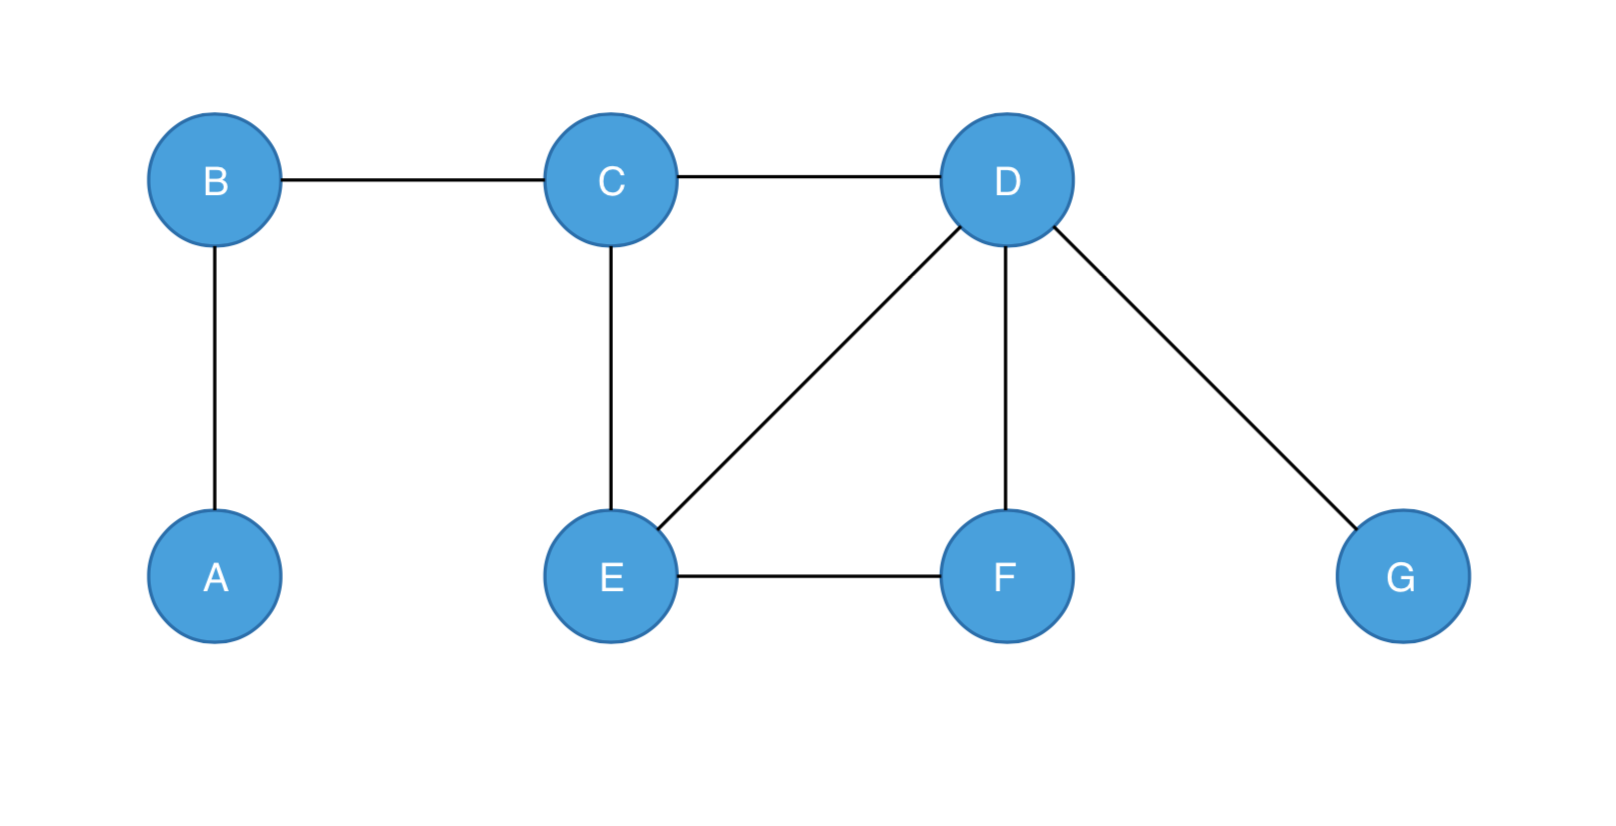
\includegraphics[height=4cm, width=9.5cm]{../images/undirected.png}
              \caption{Undirected graph}
          \end{figure}
    \item \textbf{Directed graph}: When the set $E$ is represented as an ordered pair of vertices, it is called a directed graph or digraph. In a digraph, for some $x,y \in V(G)$, $(x,y) \neq (y,x)$.
          \begin{figure}[hbt!]
              \centering
              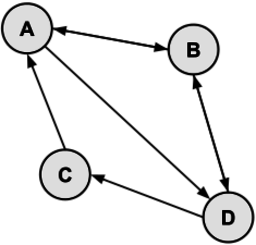
\includegraphics[height=4cm, width=7cm]{../images/directed.png}
              \caption{Directed graph}
          \end{figure}
    \item \textbf{Multigraph}: If for any given vertices $x,y \in V(G)$, $\exists$ more than one edge $(x,y)$, then it is called a multigraph.
          \begin{figure}[hbt!]
              \centering
              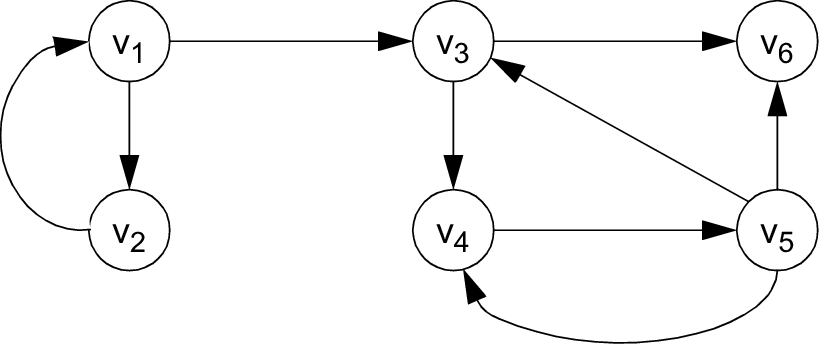
\includegraphics[height=4cm, width=9.5cm]{../images/multi.png}
              \caption{Multigraph}
          \end{figure}
    \item \textbf{Pseudograph}: If for any given vertex, $x \in V(G)$, $\exists$ an edge $(x,x)$, that is, there is some edge $e$ that connects some vertex $x$ to itself.
          \begin{figure}[hbt!]
              \centering
              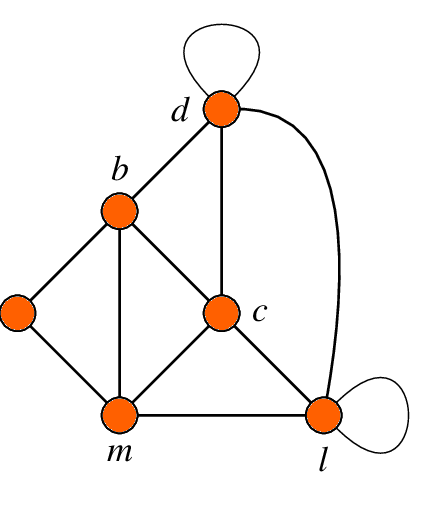
\includegraphics[height=3.82cm, width=7cm]{../images/pseudo.png}
              \caption{Pseudograph}
          \end{figure}
    \item \textbf{Hypergraph}: If the edges of a graph are arbitrary subsets of vertices it is called hypergraph.
          \begin{figure}[hbt!]
              \centering
              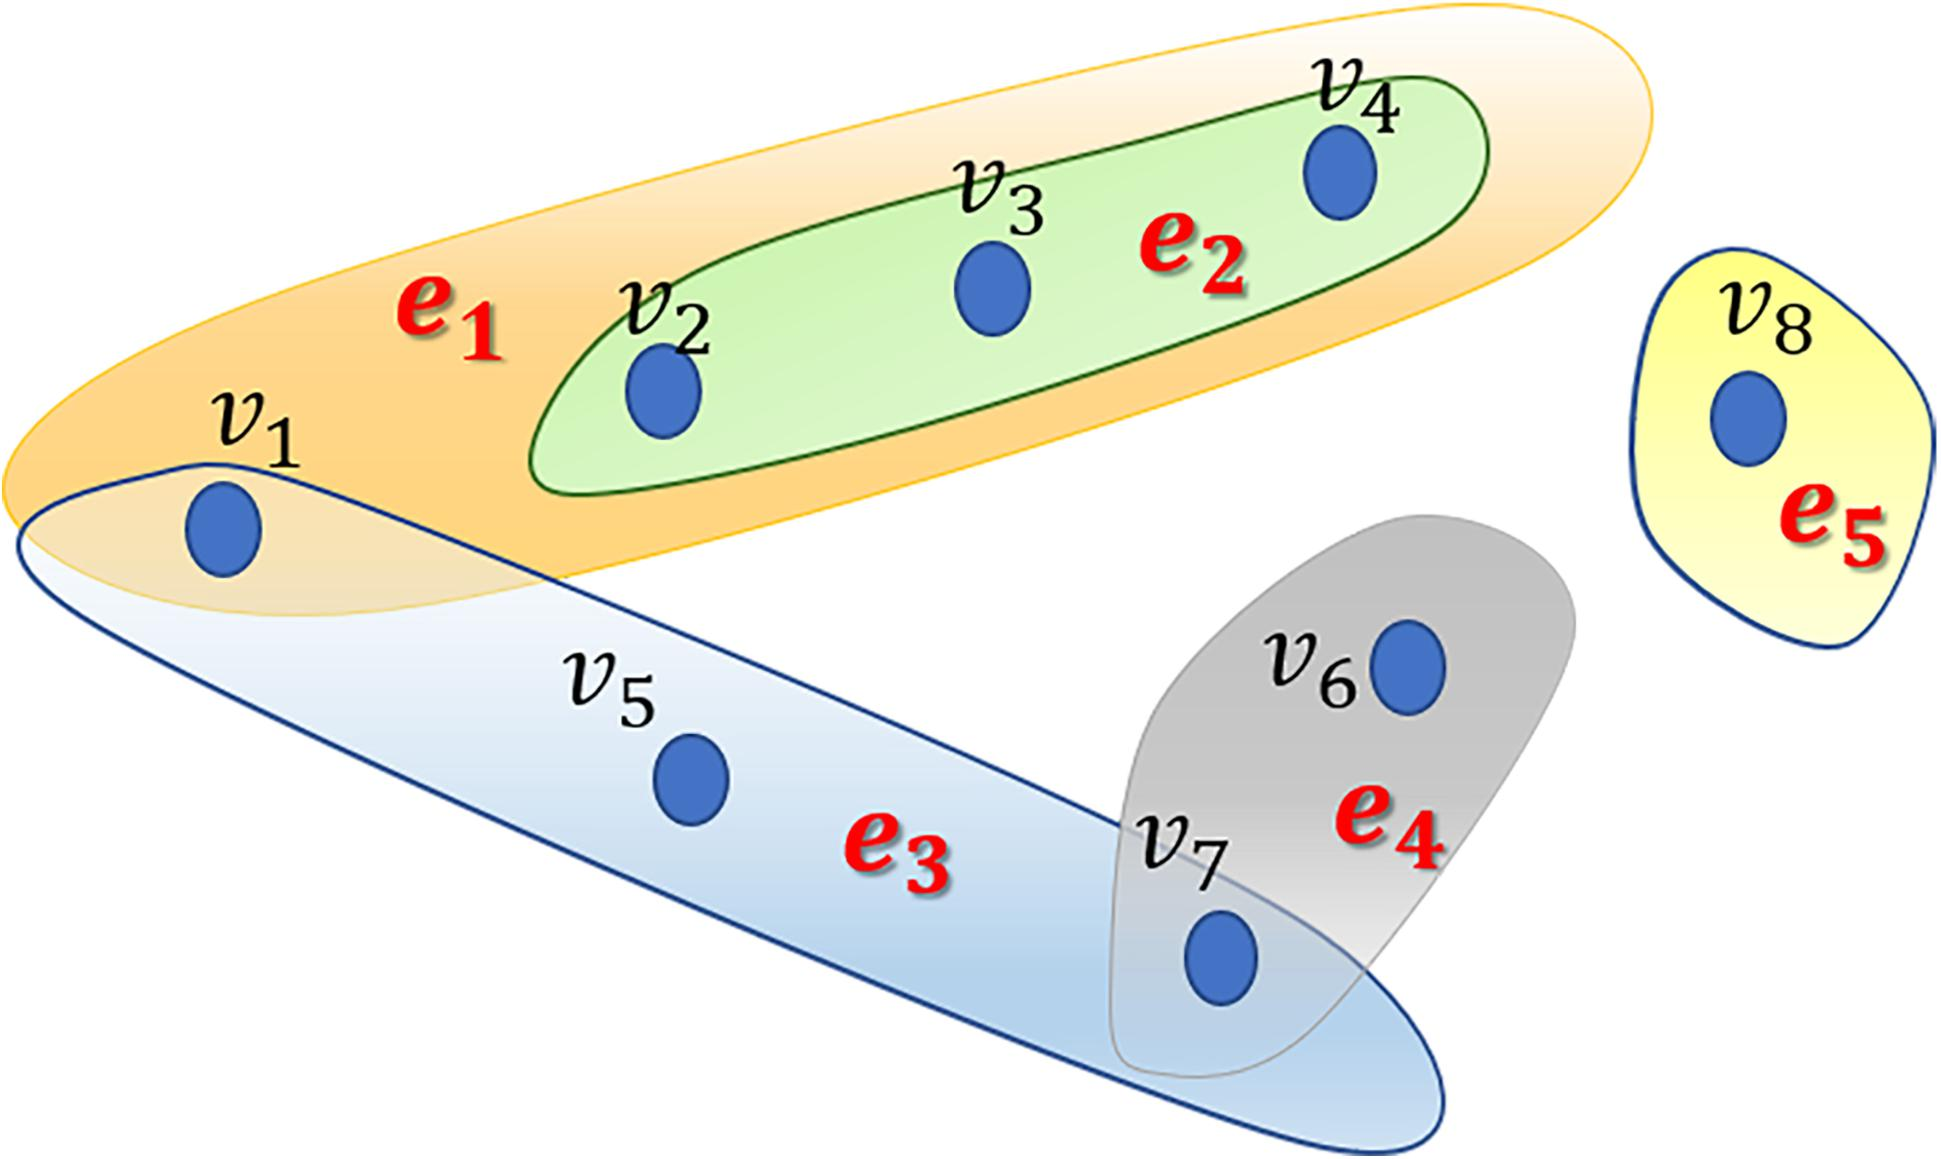
\includegraphics[height=4cm, width=9.5cm]{../images/hyper.jpg}
              \caption{Hypergraph}
          \end{figure}
    \item \textbf{Infinite graph}: If the set $V$ or $E$ is infinite then it is called infinite graph.
\end{enumerate}

Next, we go on to define some important terminologies, that we will be using throughout the length of these notes.
\begin{defn}
    The neighbourhood of a vertex $v$ in some graph G, denoted by $N(v)$, is the set of vertices adjacent to $v$.\\
    $N(v) = \{x \in V(G) \mid (v,x) \in E(G)\}$
\end{defn}

We also point out some basic ideas.
\begin{defn}
    The cardinality of $V(G)$ is called the order of the graph. Similarly, the cardinality of $E(G)$ is called the size of the graph.
\end{defn}

\begin{defn}
    The degree of a vertex $v$ in the graph G is defined as the cardinality of $N(v)$. It is denoted by $deg(v)$.
\end{defn}

We introduce two more notations:
\begin{itemize}
    \item The maximum degree of a graph G is denoted by $\Delta(G)$.\\
          $\Delta(G) = \max\{deg(v) \mid v \in V(G)\}$
    \item The minimum degree of a graph G is denoted by $\delta(G)$.\\
          $\delta(G) = \min\{deg(v) \mid v \in V(G)\}$
\end{itemize}

Now, we will state one of the famous, useful, and most basic theorems.
\begin{thm}
    In a graph $G$, the sum of the degrees of vertices is equal to twice the number of edges.\\
    $2 \times |E(G)|=\sum_{v \in V(G)}deg(v)$
\end{thm}

The proof of the theorem is rather intuitive and we leave it as an exercise for the reader.\\

Next, we introduce two very useful concepts, namely, vertex deletion and edge deletion.\\

$G-v$ represents the graph G obtained after removing vertex $v$ and all edges incident with $v$ from $G$. This is the concept of vertex deletion.\\

Furthermore, we present the concept of edge deletion. $G-e$ represents the graph $G$ after removing the edge $e$ but it's end vertices remain.\\

Moreover, there is another way of edge deltetion. $G/e$ represents the graph $G$ after removing edge $e$ and it's end vertices $v_1$ and $v_2$ are merged into a single vertex $v$. In the graph $G$, every edge incident on either $v_1$ or $v_2$, is now incident on $v$ in the new graph $G/e$.\\

We now define the concepts of connectedness, and cut sets.\\
\begin{defn}
    A graph is connected if we can travel from one vertex to another via the edges.
\end{defn}

\begin{defn}
    Each maximal connected piece of a graph is called a connected component.
\end{defn}

\begin{defn}
    If the deletion of a vertex $v$ from a graph $G$ causes the connected components to increase, then $v$ is called a cut vertex.
\end{defn}

\begin{defn}
    If the deletion of an edge $e$ from a graph $G$ causes the connected components to increase, then $e$ is called a cut edge or a bridge.
\end{defn}

\begin{defn}
    If a proper subset $S$ of $V(G)$ makes $G-S$ disconnected then $S$ is called a vertex cut set.
\end{defn}

\begin{defn}
    The connectivity of a graph $G$ is defined as the minimum size of a cut set of $G$. It is dented by $\kappa(G)$.
\end{defn}

Next, we go on to define few more types of graphs.

\begin{enumerate}
    \item The complement of a graph $G$, is defined as the graph on $n$ vertices which has all the possible vertices $(x,y) \notin E(G)$.
    \item The line graph of a graph $G$, is defined as the graph $L(G)$, where each edge in $G$ is represented by a vertex in $L(G)$ and an edge exists in between two vertices of $L(G)$ iff the corresponding edges in $G$ share a vertex.
    \item A regular graph is defined as a graph whose every vertex has equal degree.
    \item A bipartite graph is defined as a graph whose vertices can be divided into two partite sets $X$ and $Y$, such that no two vertices in a partite set are adjacent to each other.
    \item A graph $H$ is called the subgraph of a graph $G$ if $V(H) \subseteq V(G)$ and $E(H) \subseteq E(G)$.
\end{enumerate}

\begin{defn}[Graph homomorphism and isomorphism]
    Suppose $G,H$ are two graphs. A function $\phi : V(G) \to V(H)$ is said to be a {\em graph homomorphism} if $x \sim y$ implies $\phi(x) \sim \phi(y).$ $\phi$ is said to be an {\em isomorphism} if $\phi$ is a bijection and $x \sim y$ iff $\phi(x) \sim \phi(y)$ i.e., $\phi, \phi^{-1}$ are graph homomorphisms. $G$ and $H$ are {\em isomorphic} ($G \cong H$) if there exists an isomorphism between $G$ and $H$. An {\em  automorphism} is an isomorphism $\phi :G \to G$.
\end{defn}

That's all the basic definitions we will be needing. Further on, we will be introducing various interesting ideas and in our Random Graphs WRP, these ideas will be of essesnce.

\end{document}